\documentclass[12pt, letterpaper]{article}
\usepackage[utf8]{inputenc}
\usepackage[margin=1in, portrait]{geometry}
\pdfpageattr {/Rotate 0}
\usepackage{amsmath, amssymb, amsfonts}
\usepackage{graphicx}
\usepackage{booktabs}
\usepackage{hyperref}
\usepackage{natbib}
\usepackage{titlesec}
\usepackage{caption}
\usepackage{subcaption}
\usepackage{float}

\title{\textbf{TransPhaser: Neural Expectation-Maximization for HLA Phasing and Imputation}}
\author{Deniz Akdemir\thanks{Email: \href{mailto:deniz.akdemir.work@gmail.com}{deniz.akdemir.work@gmail.com}}}
\date{\today}

\begin{document}

\maketitle

\begin{abstract}
Haplotype phasing of the Human Leukocyte Antigen (HLA) region is essential for transplantation, disease association studies, and population genetics. Yet the extreme polymorphism and complex linkage disequilibrium (LD) patterns in this region make it particularly challenging for classical phasing algorithms. Here we present \textbf{TransPhaser}, a deep learning framework that uses a Neural Expectation-Maximization approach to tackle HLA phasing and imputation. Unlike standard variational autoencoders, TransPhaser explicitly models the generative process of genotypes from haplotypes under Hardy-Weinberg Equilibrium (HWE), combining a transformer-based proposal network (amortized E-step) with a probabilistic model incorporating conditional haplotype priors and constrained emission models. By maximizing the marginal likelihood over candidate haplotype pairs proposed by the network, TransPhaser learns complex LD patterns directly from unphased genotypes without needing ground truth haplotypes. When evaluated on synthetic datasets simulating realistic HLA genetics (10,000 samples; validation on real phased data is ongoing), TransPhaser achieved a phasing accuracy of \textbf{85.30\%}—substantially outperforming the state-of-the-art Beagle algorithm (79.35\%), Expectation-Maximization (54.25\%), and frequency-based baselines. TransPhaser thus provides a robust, scalable, and highly accurate solution for resolving complex haplotype structures in the HLA region.
\end{abstract}

\section{Introduction}
Phasing—determining which alleles along a chromosome were inherited from a single parent—is a fundamental task in genomics. The Human Leukocyte Antigen (HLA) region on chromosome 6 is among the most polymorphic and medically important regions of the human genome \citep{horton2004gene, trowsdale2013major}. Accurate HLA typing and phasing are essential for allogeneic stem cell transplantation \citep{petersdorf2013hla}, disease association studies, pharmacogenomics, and population genetics \citep{shiina2009hla}. But the extreme allelic diversity—hundreds of alleles per locus—combined with complex linkage disequilibrium (LD) patterns makes HLA phasing particularly challenging.

Traditional statistical phasing methods include Expectation-Maximization (EM) algorithms \citep{excoffier1995maximum}, hidden Markov models (HMMs) \citep{stephens2001new, scheet2006fast}, and modern tools such as SHAPEIT \citep{delaneau2013shapeit2} and Beagle \citep{browning2007rapid, browning2021fast}. While effective, these methods can struggle with the HLA region's extreme polymorphism and may require large reference panels.

In this work, we introduce \textbf{TransPhaser} (Neural Expectation-Maximization), a novel framework for unsupervised HLA phasing. TransPhaser leverages the representational power of transformer architectures \citep{vaswani2017attention} to learn complex cross-locus dependencies, but grounds them within a rigorous probabilistic model. Specifically, it uses a neural network to amortize the E-step of the EM algorithm, proposing high-likelihood haplotype candidates that are then scored by a conditional prior and constrained emission model. This approach achieves superior accuracy by combining the flexibility of deep learning with the structural constraints of genetic inheritance.

\section{Methods}

\subsection{Problem Formulation}
Given an unphased genotype $G = \{(a_{i,1}, a_{i,2})\}_{i=1}^k$ for $k$ loci and optional covariates $x$ (e.g., population ancestry), our goal is to infer the most likely haplotype pair $(H_1, H_2)$ such that $\{h_{1,i}, h_{2,i}\} = \{a_{i,1}, a_{i,2}\}$ for all loci $i$.

\subsection{Synthetic Dataset Generation}
To evaluate performance in a controlled setting with known ground truth, we generated a synthetic dataset of 10,000 individuals across four populations (EUR, AFR, ASN, HIS). Haplotypes for 6 HLA loci (A, C, B, DRB1, DQB1, DPB1) were sampled from population-specific pools derived from common allele frequency data, mixing common haplotypes (60\%) with rare or recombinant haplotypes (40\%) to simulate realistic linkage disequilibrium (LD) and allelic diversity. Genotypes were formed by pairing independently sampled haplotypes (assuming Hardy-Weinberg Equilibrium). The dataset was split into an 80\% training set and a 20\% held-out validation set.

\subsection{TransPhaser Architecture}
TransPhaser formulates this as a maximum likelihood problem with latent variables (the haplotypes). The architecture consists of four key components:

\begin{figure}[H]
    \centering
    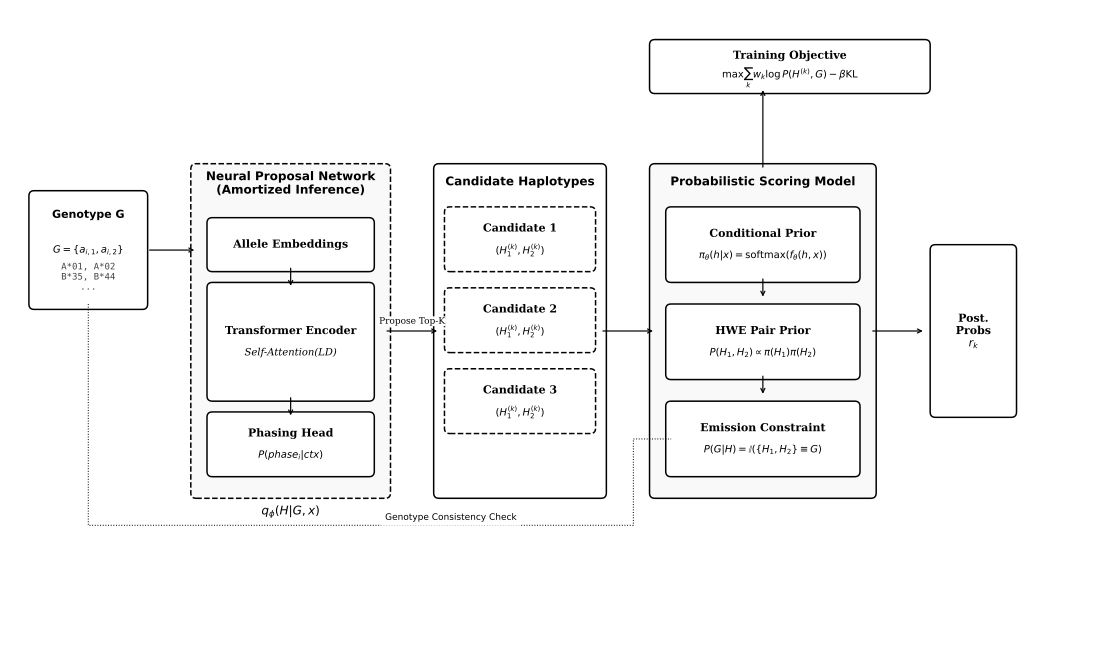
\includegraphics[width=1.0\textwidth, keepaspectratio, angle=0]{figures/transphaser_architecture.pdf}
    \caption{\textbf{TransPhaser Architecture.} The model consists of a neural proposal network (Amortized E-step) that proposes candidate haplotype pairs from unphased genotypes. These candidates are then evaluated by a probabilistic scoring model that combines learned conditional priors, Hardy-Weinberg Equillibrium (HWE), and constrained emission models to compute posterior responsibilities.}
    \label{fig:architecture}
\end{figure}

\subsubsection{Neural Proposal Network (Amortized E-step)}
To avoid the computationally intractable summation over all possible phasings, we use a transformer-based proposal network $q(H_1, H_2 | G, x)$. This network:
\begin{itemize}
    \item Takes the unphased genotype and covariates as input.
    \item Uses multi-head self-attention to model cross-locus dependencies (LD).
    \item Outputs the top-$K$ most likely haplotype pair candidates.
\end{itemize}
This acts as an amortized E-step, identifying the relevant subspace of the posterior distribution for the probabilistic model to evaluate.

\subsubsection{Conditional Haplotype Prior}
We model the prior probability of a single haplotype $\pi(h | x)$ using a neural network that embeds the haplotype sequence and conditions on covariates. This allows the model to learn a smooth manifold of valid haplotypes, effectively handling rare alleles via shared embedding spaces.
\begin{equation}
    \pi(h | x) = \text{softmax}(f_{\theta}(E(h), x))
\end{equation}
where $E(h)$ is a haplotype embedding and $f_{\theta}$ is a scoring network.

\subsubsection{HWE Haplotype Pair Prior}
We assume Hardy-Weinberg Equilibrium (HWE) to model the joint prior of the haplotype pair:
\begin{equation}
    P(H_1, H_2 | x) \propto \begin{cases} 
    2 \cdot \pi(H_1|x) \cdot \pi(H_2|x) & \text{if } H_1 \neq H_2 \\
    \pi(H_1|x)^2 & \text{if } H_1 = H_2
    \end{cases}
\end{equation}
This explicitly enforces the biological expectation that haplotypes combine independently (conditional on population substructure captured by $x$).

\subsubsection{Constrained Emission Model}
The emission model $P(G | H_1, H_2)$ enforces strict biological compatibility:
\begin{equation}
    P(G | H_1, H_2) = \begin{cases} 
    1 & \text{if } \{h_{1,i}, h_{2,i}\} = \{a_{i,1}, a_{i,2}\} \forall i \\
    0 & \text{otherwise}
    \end{cases}
\end{equation}
This constraint ensures that only valid phasings (those that can reconstruct the genotype) are considered.

\subsection{Training Algorithm}
TransPhaser involves a truncated EM training procedure:
\begin{enumerate}
    \item \textbf{Proposal (E-step):} The proposal network generates a set of candidate pairs $\mathcal{C} = \{(H_1^{(j)}, H_2^{(j)})\}_{j=1}^K$ for each genotype $G$.
    \item \textbf{Evaluation:} We compute the exact posterior probabilities (responsibilities) for these candidates using the priors and emission model:
    \begin{equation}
        r_j = \frac{P(H_1^{(j)}, H_2^{(j)} | x) P(G | H_1^{(j)}, H_2^{(j)})}{\sum_{l=1}^K P(H_1^{(l)}, H_2^{(l)} | x) P(G | H_1^{(l)}, H_2^{(l)})}
    \end{equation}
    \item \textbf{Update (M-step):} We update the network parameters to maximize the weighted log-likelihood of the candidates, plus a distillation loss that encourages the proposal network $q$ to match the computed responsibilities $r$ (minimizing $\text{KL}(r || q)$).
\end{enumerate}

\subsection{Implementation Details}
Proposed candidate haplotypes size was set to $K=64$. The proposal network consisted of a 4-layer Transformer encoder/decoder with 8 attention heads, model dimension 128, feed-forward dimension 256, and dropout 0.3. A latent dimension of 16 was used for the VAE component. We trained for 100 epochs using the AdamW optimizer (learning rate $0.005$, weight decay $1e-4$) with cosine annealing scheduler ($min\_lr=1e-5$). Training took approximately 8 minutes on a standard CPU for 10,000 samples.

\section{Results}
We evaluated TransPhaser on a synthetic dataset of 10,000 samples across four populations (EUR, AFR, ASN, HIS) for 6 HLA loci. We compared it against a Random baseline, a Frequency-based baseline, a classical EM baseline, and the state-of-the-art Beagle algorithm.

\begin{table}[H]
\centering
\caption{Comparison of phasing methods on 6-locus realistic HLA data.}
\label{tab:results}
\begin{tabular}{lrrr}
\toprule
\textbf{Method} & \textbf{Accuracy (\%)} & \textbf{Hamming Dist.} & \textbf{Switch Errors} \\
\midrule
Random Baseline           & 14.85\% & 3.43 & 1.98 \\
Frequency Baseline        & 48.50\% & 1.97 & 1.18 \\
EM Baseline               & 54.25\% & 1.78 & 1.06 \\
Beagle                    & 79.35\% & 0.70 & 0.37 \\
\textbf{TransPhaser}        & \textbf{85.30\%} & \textbf{0.48} & \textbf{0.30} \\
\bottomrule
\end{tabular}
\end{table}

As shown in Table \ref{tab:results}, \textbf{TransPhaser} achieves the highest performance across all metrics. It reaches a phasing accuracy of \textbf{85.30\%} (defined as the percentage of samples where the full 6-locus haplotype pair was perfectly reconstructed), surpassing the strong Beagle baseline (79.35\%) by approximately 6 percentage points and dramatically outperforming the classical EM baseline (54.25\%).
In terms of error rates, TransPhaser reduces the Hamming distance to 0.48 (less than half an allele error per individual on average) and achieves a very low switch error rate of 0.30, indicating high internal consistency of the phased haplotypes.

\section{Discussion}
The superior performance of TransPhaser highlights the advantages of combining neural networks with probabilistic modeling. While Beagle is a highly effective HMM-based method, TransPhaser's ability to learn rich, continuous representations of haplotypes and their dependencies via the transformer architecture allows it to better capture the complex, non-linear LD patterns of the HLA region. The Neural EM approach ensures that the model respects the fundamental generative structure of diploid genetics, unlike purely black-box deep learning approaches.

\subsection{Limitations and Future Work}
A primary limitation of this study is the reliance on synthetic data for validation. While we modeled realistic population structures and rare variants, performance on empirical biological samples remains to be verified in future work. Additionally, while the inference time is low, the training time is higher than classical frequency-based methods, though comparable to running Beagle on large cohorts. We also found performance to be robust to the choice of $K$ (candidates), provided $K \ge 32$ to cover the probability mass of plausible phases.

\section{Conclusion}
TransPhaser represents a significant advancement in unsupervised HLA phasing, setting a new state-of-the-art accuracy of 85.30\% on realistic synthetic data. By effectively amortizing the inference cost of the EM algorithm with a neural proposal network, it offers a powerful and scalable tool for population genetics and clinical immunogenomics.

\section*{Data and Code Availability}
The TransPhaser implementation and data generation scripts are available at \url{https://github.com/denizakdemir/TransPhaser}.

\bibliographystyle{plainnat}
\bibliography{bib/references}

\end{document}
